\chapter{Implementácia}
Táto kapitola popisuje čitateľovi samotnú implementáciu aplikácie. Čitateľ sa oboznámi s použitými nástrojmi pri tvorení aplikácie a s postupom implementácie frontendovej a backendovej časti. Prvým bodom implementácie bolo vytvorenie zložky mono-repozitára zahrňujúci obe časti aplikácie.

\section{Git a GitHub}
Pred začatím písania zdrojového kódu sa najprv spojazdnil verzovací systém Git cez GitHub. Cieľom bolo verzovanie samotného zdrojového kódu aj dokumentácie. Pre jednoduchšiu orientáciu v repozitároch sa vytvorila GitHub organizácia, ktorá obsahuje monorepozitár pre zdrojový kód a repozitár pre dokumentáciu na jednom mieste. Monorepozitár je repozitár obsahujúci viacero projektov, v tomto prípade projekt klienta a servera. Organizácia aj repozitáre sú verejne dostupné pod odkazom:
    \begin{verbatim}
        https://github.com/AdamAbrahaamBC
    \end{verbatim}

GitHub ponúka projektom organizačnú tabuľku(project board). Tabuľka pomáha v organizovaní úloh a poskytuje jednoduchší prehľad projektu. Môže mať ľubovolný počet kolóniek, do ktorých sa prideľujú jednotlivé úlohy. V tomto projekte bolo postačujúce vytvorenie troch kolóniek. Kolónka \texttt{To Do} obsahuje ešte nezačaté úlohy, kolónka \texttt{In progress} úlohy, ktoré sa práve riešia a kolónka \texttt{Done} už dokončené a zatvorené úlohy. Pri vytvorení novej úlohy sa úloha automaticky priradí do kolónky \texttt{To Do}. Pri zvolení následujúcej úlohy musí byť manuálne premiestnená do kolónky \texttt{In Progress} a pri jej zatvorení sa automaticky premiestni do kolónky \texttt{Done}.


K jednotlivým úlohám sú pridelené štítky. Štítky označujú o aký typ úlohy sa jedná. Dostupné štítky projektu sú nasledujúce.

    \begin{itemize}
        \item\textbf{backend} - označuje úlohy týkajúce sa backendu
        \item\textbf{frontend} - označuje úlohy týkajúce sa frontendu
        \item\textbf{db} - označuje úlohy na databáze
        \item\textbf{bug} - označuje úlohy obsahujúce chybu v aplikácii
        \item\textbf{todo} - označuje zatiaľ nezačaté úlohy
        \item\textbf{done} - označuje dokončené úlohy
    \end{itemize}
    
    \begin{figure}[!hbt]
        \centering
        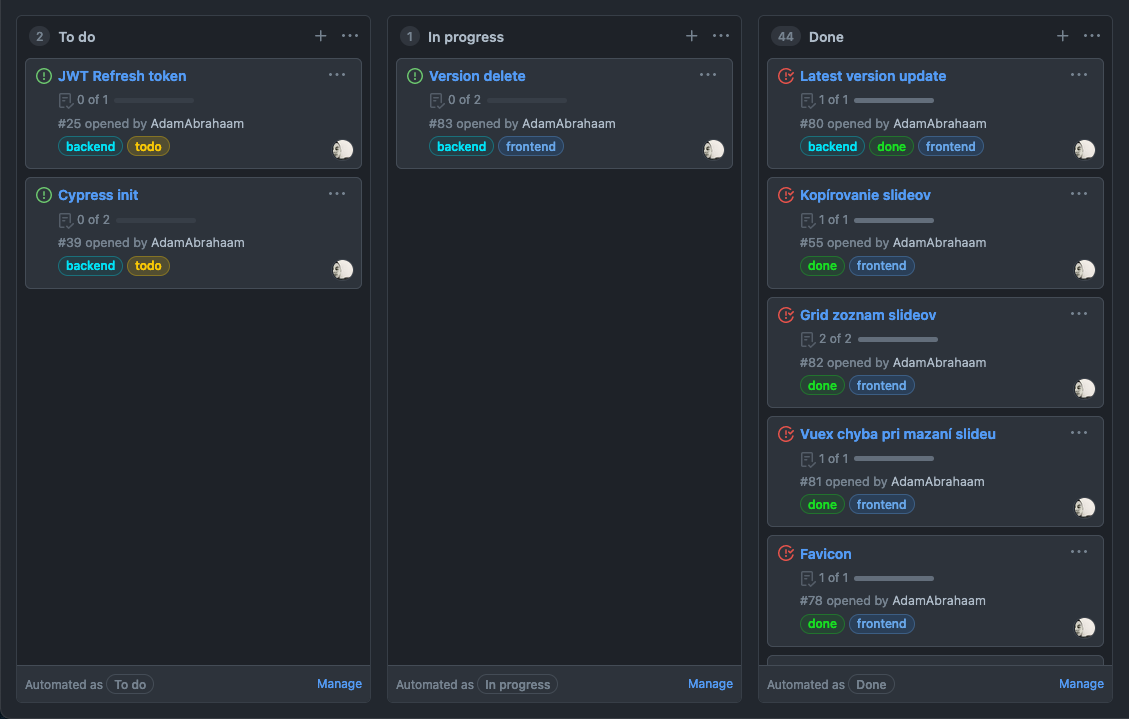
\includegraphics[scale=0.3]{obrazky/board.png}
        \caption{Organizačná tabuľka projektu}
        \label{pic:board}
    \end{figure}

\section{Implementácia frontendu}
Implementácia frontendu sa začala stiahnutím \texttt{Node.js}. Node.js obsahuje nástroj \texttt{npx} pre spúšťanie balíčkov. Pomocou npx sa vytvoril Nuxt.js projekt cez terminálový príkaz: \texttt{npx create-nuxt-app <názov-projektu>}. 

\vspace{5mm}
Po zadaní príkazu sa spustí sprievodca inštalácie, kde sa zvolil:
    \begin{itemize}
        \item správca balíčkov \texttt{npm}
        \item podpora pre \texttt{TypeScript}
        \item \texttt{Buefy} framework pre užívateľské prostredie
        \item komunikačný modul \texttt{axios}
        \item analyzačný nástroj zdrojového kódu \texttt{ESLint} 
        \item \texttt{jednostránkový} typ aplikácie(SPA)
    \end{itemize}
    
\vspace{5mm}
Balík Composition API je potrebné nainštalovať cez npm pomocou príkazu \texttt{npm install @nuxtjs/composition-api --save} a treba ho pridať medzi Nuxtom používané moduly v súbore \texttt{nuxt.config.js}.

Súbor \texttt{nuxt.config.ts} treba hneď na začiatku zvýrazniť. Je to súbor obsahujúci konfigurácie aplikácie. Nastavujú sa v ňom vlastnosti hlavičky aplikácie, ako názov, meta značky a ikonka. Obsahuje nastavenia smerovania, TypeScriptu, autentifikačného modulu, globálnych CSS súborov a ostatných rozširovacích modulov.

Nuxt.js udáva jednoduchý štartovací bod pre vývoj aplikácie. Po inicializácii projektu skonštruuje štruktúru aplikácie, ktorá je doplnená adresármi \texttt{composable} a \texttt{models}. štruktúru aplikácie dokopy tvoria nasledujúce adresáre:

\vspace{5mm}
\dirtree{%
.1 /client.
.2 /\.nuxt.
.2 /assets.
.2 /components.
.2 /composable.
.2 /dist.
.2 /layouts.
.2 /models.
.2 /node\_modules.
.2 /pages.
.2 /plugins.
.2 /store.
}
\vspace{5mm}

\subsection{Autentifikácia užívateľov}
Autentifikáciu užívateľov má na starosti autentifikačný nuxt modul. Modul sa nainštaluje cez npm, príkazom \texttt{npm install --save-exact @nuxtjs/auth-next} a pridal do nuxt konfiguračného súboru medzi moduly. Autentifikačný modul vyžaduje inštaláciu nuxt modulu \texttt{axios} pre HTTP komunikáciu. 

Middleware je globálne nastavený v nuxt konfiguračnom súbore na každú jednu trasu aplikácie okrem stránky prihlasovania, registrovania a zobrazenia prezentácie v prezentačnom móde. Na týchto stránkach je middleware manuálne vypnutý a sú dostupné bez autentifikácie. Neprihlásený užívateľ pri navštívení stránky, ktorá autentifikáciu vyžaduje je automaticky presmerovaný na prihlasovaciu stránku.

Modul funguje na báze schém. Schémy definujú logiku autentifikácie. Projekt môže obsahovať viacero schém pre rôzne typy prihlasovania, napríklad cez Facebook, Google, atď. V aplikácii je implementovaná lokálna schéma na báze JWT tokenov. Jej konfigurácia sa nachádza v konfiguračnom súbore. 

Modul poskytuje aplikačné rozhranie cez kľúčové slovo \$auth, ktoré je globálne dostupné cez kontext aplikácie. Prihlasuje sa cez funkciu \texttt{\$auth.loginWith('local', { data: PRIHLASOVACIE\_ÚDAJE })}. Modul pošle na prihlasovací koncový bod prihlasovacie údaje. Pri úspešnom prihlásení API vráti v HTTP odpovedi autentifikačný token užívateľa, ktorý sa uloží do koláčov(cookies) aplikácie a modul si automaticky vypýta údaje o užívateľovi podľa tokenu. Údaje užívateľa sú dostupné cez objekt \texttt{\$auth.user}. Odhlasuje sa cez \texttt{\$auth.logout()}.

\subsection{Smerovanie a stránky}
Smerovanie vo Vue.js sa rieši cez balík \texttt{vue-router}. Jednotlivé vlastnosti trias ako URI, komponenta pre vykreslenie a  potomky je potrebné nakonfigurovať v konfiguračnom súbora. 

Nuxt.js uľahčuje vývoj aj v tomto smere. Pomocou frameworku nie je potrebné konfigurovať trasy, Nuxt.js zoberie všetky zložky a súbory z adresára \texttt{pages} a skonštruuje smerovanie aplikácie automaticky. Každá zložka v adresári je samostatná trasa, ktorá obsahuje súbor \texttt{index.js} zahrňujúca komponentu stránky. Každá komponenta stránky je samostatná Vue.js komponenta so špeciálnymi atribútmi a funkciami. Zložky môžu obsahovať ďalšie vnorené zložky pre vnorené trasy. Zložky pomenované s podčiarkovníkom(\_) na začiatku sú dynamické, ich hodnota sa mení. Dynamické stránky v aplikácii sa využívajú pre konkrétnu prezentáciu \texttt{/presentation/\_id} a pre konkrétnu verziu prezentácie \texttt{/presentation/\_id/\_version}, kde sa tieto názvy menia podľa potreby. Obsah adresára:

\vspace{5mm}
\dirtree{%
.1 /pages.
.2 /login.
.3 index.vue.
.2 /register.
.3 index.vue.
.2 /presentation.
.3 /new.
.4 /preview.
.5 index.vue.
.4 index.vue.
.3 /\_id.
.4 /\_version.
.5 /preview.
.6 index.vue.
.5 index.vue.
.2 index.vue.
}
\vspace{5mm}

\subsection{Perzistované úložisko}
Uchovávanie jednotlivých stavov aplikácie je implementované cez modul \texttt{Vuex}. Aplikácia uchováva neuložené zmeny prezentácie a skopírovanú stránku. Pri opustení editora bez uložení zmien aplikácia upozorní užívateľa, že sa jeho zmeny môžu stratiť. Môže nastať situácia pri tvorbe prezentácie, keď sa z technických dôvodov aplikácia, alebo prehliadač zatvorí. V takomto prípade sa užívateľovi nové zmeny zachovajú a bude ich mať dostupné keď sa vráti do editora danej prezentácie a verzie. Uchovávanie skopírovanej stránky sa využíva pri skopírovaní a vložení stránky prezentácie. 

Štandardne sa uchované stavy vo Vuex po opustení aplikácie automaticky zmažú. Na perzistovanie úložiska sa využil balík \texttt{vuex-persistedstate}, pomocou ktorého sa stavy uložia do lokálneho úložiska prehliadača a sú dostupné aj pri znovu navštívení aplikácie.

Podľa zásady, stavy sa upravujú iba cez mutácie v úložisku. Mutácia sa volajú cez akcie, ktoré sú dostupné cez kľúčové slovo \texttt{store} v kontexte aplikácie. Implementácia samotného úložiska sa nachádza v adresári \texttt{store}. Zložka \texttt{presentation} obsahuje všetky potrebné súbory pre beh úložiska.

    \begin{itemize}
        \item súbor \texttt{index.ts} obsahuje uložené stavy prezentácie:
        \begin{itemize}
            \item \texttt{presentation} posledná upravovaná prezentácia
            \item \texttt{copiedSlide} skopírovaná stránka prezentácie
        \end{itemize}
        
        \item súbor \texttt{mutations.ts} obsahuje mutácie stavov:
        \begin{itemize}
            \item \texttt{SET\_PRESENTATION} pridelenie hodnoty stavu prezentácie
            \item \texttt{SET\_COPIED\_SLIDE} pridelenie hodnoty stavu skopírovanej stránky
        \end{itemize}
        
        \item súbor \texttt{actions.ts} obsahuje metódy akcií nad mutáciami:
        \begin{itemize}
            \item \texttt{SAVE\_PRESENTATION} uloženie prezentácie do úložiska\\(volanie mutácie SET\_PRESENTATION s hodnotou prezentácie)
            \item \texttt{REMOVE\_PRESENTATION} vymazanie prezentácie z úložiska\\(volanie mutácie SET\_PRESENTATION s hodnotou \texttt{null})
            \item \texttt{COPY\_SLIDE} uloženie skopírovanej stránky do uložiska\\(volanie mutácie SET\_COPIED\_SLIDE s hodnotou danej stránky)
        \end{itemize}
        
        \item súbor \texttt{getters.ts} obsahuje metódy na vrátenie hodnôt stavov v úložisku:
        \begin{itemize}
            \item \texttt{getPresentation} vráti hodnotu stavu prezentácie
            \item \texttt{getCopiedSlide} vráti hodnotu stavu skopírovanej stránky
        \end{itemize}
    \end{itemize}
    
Pre zjednodušenie prístupu k úložisku a pre odstránenie biolerplate kódu sa vytvorila trieda \texttt{PresentationStore} v adresári \texttt{composable}. V jednotlivých komponentoch a na stránkach sa pristupuje k úložisku cez metódy tejto triedy. Trieda zapúzdruje vyššie popisované metódy akcií a metódy na vrátenie hodnôt stavov.

\subsection{Znovupoužiteľná logika}

\subsection{Zobrazovanie a upravovanie Markdown obsahu}

\subsection{Extrahovanie statickej prezentácie}